\documentclass{article}
\usepackage[utf8]{inputenc}
\usepackage{algorithm}
\usepackage{algpseudocode}
\usepackage{amsmath}
\usepackage{amssymb}
\usepackage{graphicx}

\title{Project Report \\ Cache-Aware and Cache-Oblivious Algorithms for String Sorting}
\author{Kausheya Roy \and Harshit Lalwani}
\date{May 2026}

\begin{document}

\maketitle

\section{Problem Statement}
This project studies cache-aware and cache-oblivious algorithms with the goal of designing and implementing efficient solutions for \textbf{String Sorting}. We evaluate these algorithms based on their ability to minimize I/O operations $Q(N; M; B)$ between a fast internal memory of size $M$ and a larger memory, where data is transferred in blocks of size $B$. The primary metric of success is how closely an algorithm approaches the scanning bound $Scan(N) = O(N/B)$.

\section{The Architecture Problem with Baseline Algorithms}
Standard algorithms often ignore the memory hierarchy, leading to significant performance degradation on large datasets.

\subsection{Standard Introsort (std::sort)}
Standard implementations like \texttt{std::sort} treat strings as opaque objects. When sorting $N$ strings, the algorithm performs $O(N \log N)$ comparisons. In a string context, each comparison can trigger multiple cache misses as the CPU fetches character data from arbitrary heap locations, leading to poor spatial locality and high $Q(N)$.

\subsection{Multi-key Quicksort (MKQS)}
\textbf{Idea:} MKQS partitions strings into three sets (less than, equal to, and greater than) based on the character at the current depth $d$.

\begin{algorithm}
\caption{Multi-key Quicksort ($A, lo, hi, d$)}
\begin{algorithmic}[1]
\If{$hi \leq lo$} \Return \EndIf
\State $pivot \gets char\_at(A[lo], d)$
\State Partition $A[lo \dots hi]$ into $\{< pivot, = pivot, > pivot\}$
\State \textbf{MKQS}($A, lo, lt-1, d$)
\State \textbf{MKQS}($A, lt, gt, d+1$) \Comment{Move to next character for equal partition}
\State \textbf{MKQS}($A, gt+1, hi, d$)
\end{algorithmic}
\end{algorithm}

\textbf{Problem:} While MKQS avoids re-comparing characters, it suffers from poor cache utilization during partitioning. If the dataset size $N > M$, the random-access nature of the swaps causes frequent cache line evictions.

\section{Cache-Aware Algorithm: Burstsort}
\textbf{Idea:} Burstsort uses a Trie where leaves are containers (buckets). It ensures the "Working Set" of strings being sorted fits into the cache.

\begin{algorithm}
\caption{Burstsort ($S, L$)}
\begin{algorithmic}[1]
\State Initialize Trie root with an empty bucket
\For{each string $s \in S$}
    \State Traverse Trie to find the correct leaf bucket
    \State Insert $s$ into bucket
    \If{size(bucket) $> L$} \textbf{Burst}(bucket) \EndIf
\EndFor
\State Sort each bucket using a cache-efficient baseline (e.g., MKQS)
\end{algorithmic}
\end{algorithm}

\textbf{Analysis:}
\begin{itemize}
    \item \textbf{TC:} $O(D + N \log L)$, where $D$ is the total length of distinguishing prefixes.
    \item \textbf{Q Calculation:} $Q(N) \approx O(N/B \cdot D/L)$.
    \item \textbf{Proof:} By setting $L < M$, each bucket sort occurs entirely within the cache. The I/O cost is dominated by the initial distribution (effectively a Scan) and the final sequential read of the Trie, both of which are $O(N/B)$.
\end{itemize}

\section{Cache-Aware Algorithm: MSD Radix Sort}
\textbf{Idea:} MSD Radix Sort uses a distribution-based approach, counting frequencies of characters at depth $d$ and shuffling strings into $R$ buckets.

\begin{algorithm}
\caption{MSD Radix Sort ($A, lo, hi, d, aux$)}
\begin{algorithmic}[1]
\State \textbf{Count:} Frequencies of $char\_at(s, d)$ for $s \in A[lo \dots hi]$
\State \textbf{Indices:} Transform counts into starting positions in $aux$
\State \textbf{Distribute:} Move strings from $A$ to $aux$ using indices
\State \textbf{Copy Back:} $A[lo \dots hi] \gets aux[0 \dots hi-lo]$
\State \textbf{Recurse:} For each character $r \in \text{Alphabet}$, sort sub-partitions at $d+1$
\end{algorithmic}
\end{algorithm}

\textbf{Analysis:}
\begin{itemize}
    \item \textbf{Q Calculation:} $Q(N) = O(N \cdot D/B)$ if $Alphabet\_Size < M/B$.
    \item \textbf{Proof:} Each pass is a $Scan(N)$, costing $O(N/B)$. However, if the alphabet size is too large, the write pointers for each bucket will reside in different cache lines. If the number of lines exceeds $M/B$, every write may cause a cache miss (thrashing).
\end{itemize}

\section{Cache-Oblivious Algorithm: Funnelsort (Lazy)}
\textbf{Idea:} Uses a recursive divide-and-conquer approach that is optimal without knowing $M$ or $B$. We implement a multi-way merge sort that recursively splits the input.

\begin{algorithm}
\caption{Lazy Funnelsort ($S$)}
\begin{algorithmic}[1]
\If{size($S$) fits in cache block $B$}
    \State Sort $S$ using a standard base-case sort
\Else
    \State Divide $S$ into $K = N^{1/3}$ streams
    \State \textbf{Lazy Funnelsort}(each stream)
    \State Merge streams using a $K$-way Funnel (merger)
\EndIf
\end{algorithmic}
\end{algorithm}

\textbf{Analysis:}
\begin{itemize}
    \item \textbf{Q Calculation:} $Q(N) = O(N/B \log_{M/B} N/B)$.
    \item \textbf{Proof:} Because the algorithm uses divide-and-conquer, it eventually reaches a subproblem size $n$ such that $n^2 \leq M$. At this point, the subproblem and its merge buffers fit entirely in the cache, and all subsequent recursive calls incur zero further I/O misses. This recursive structure makes it optimal for any $M$ and $B$.
\end{itemize}

\section{Datasets}
To rigorously test the architecture-friendliness, we utilized two primary dataset categories:

\subsection{Synthetic Datasets}
Generated using C++ pseudo-random generators to control specific performance variables.
\begin{itemize}
    \item \textbf{Random:} Strings of lengths 4--24 with uniform character distribution to test $N \log N$ behaviors.
    \item \textbf{Prefix-Heavy:} Strings sharing long common prefixes (e.g., "cache\_aware\_1", "cache\_aware\_2") to force algorithms to process deeper distinguishing prefixes ($D$) and stress the $Q$ complexity.
\end{itemize}

\subsection{Real-World Dataset: Wikipedia Titles}
A collection of 5 million titles from English Wikipedia. This dataset represents real-world "Long Tail" distributions and heavy prefix overlaps, providing a benchmark for how algorithms handle actual data skewedness.

\section{Experiments and Performance Analysis}
We conducted benchmarks across varying problem sizes $N = \{10^5, 10^6, 5 \times 10^6\}$.

\subsection{Time Performance per Element}
We plotted the execution time per element (in $\mu s$) against $N$ for all algorithms. Normalizing by $N$ reveals cache-related performance degradation as problem sizes grow.

\begin{figure}[h]
    \centering
    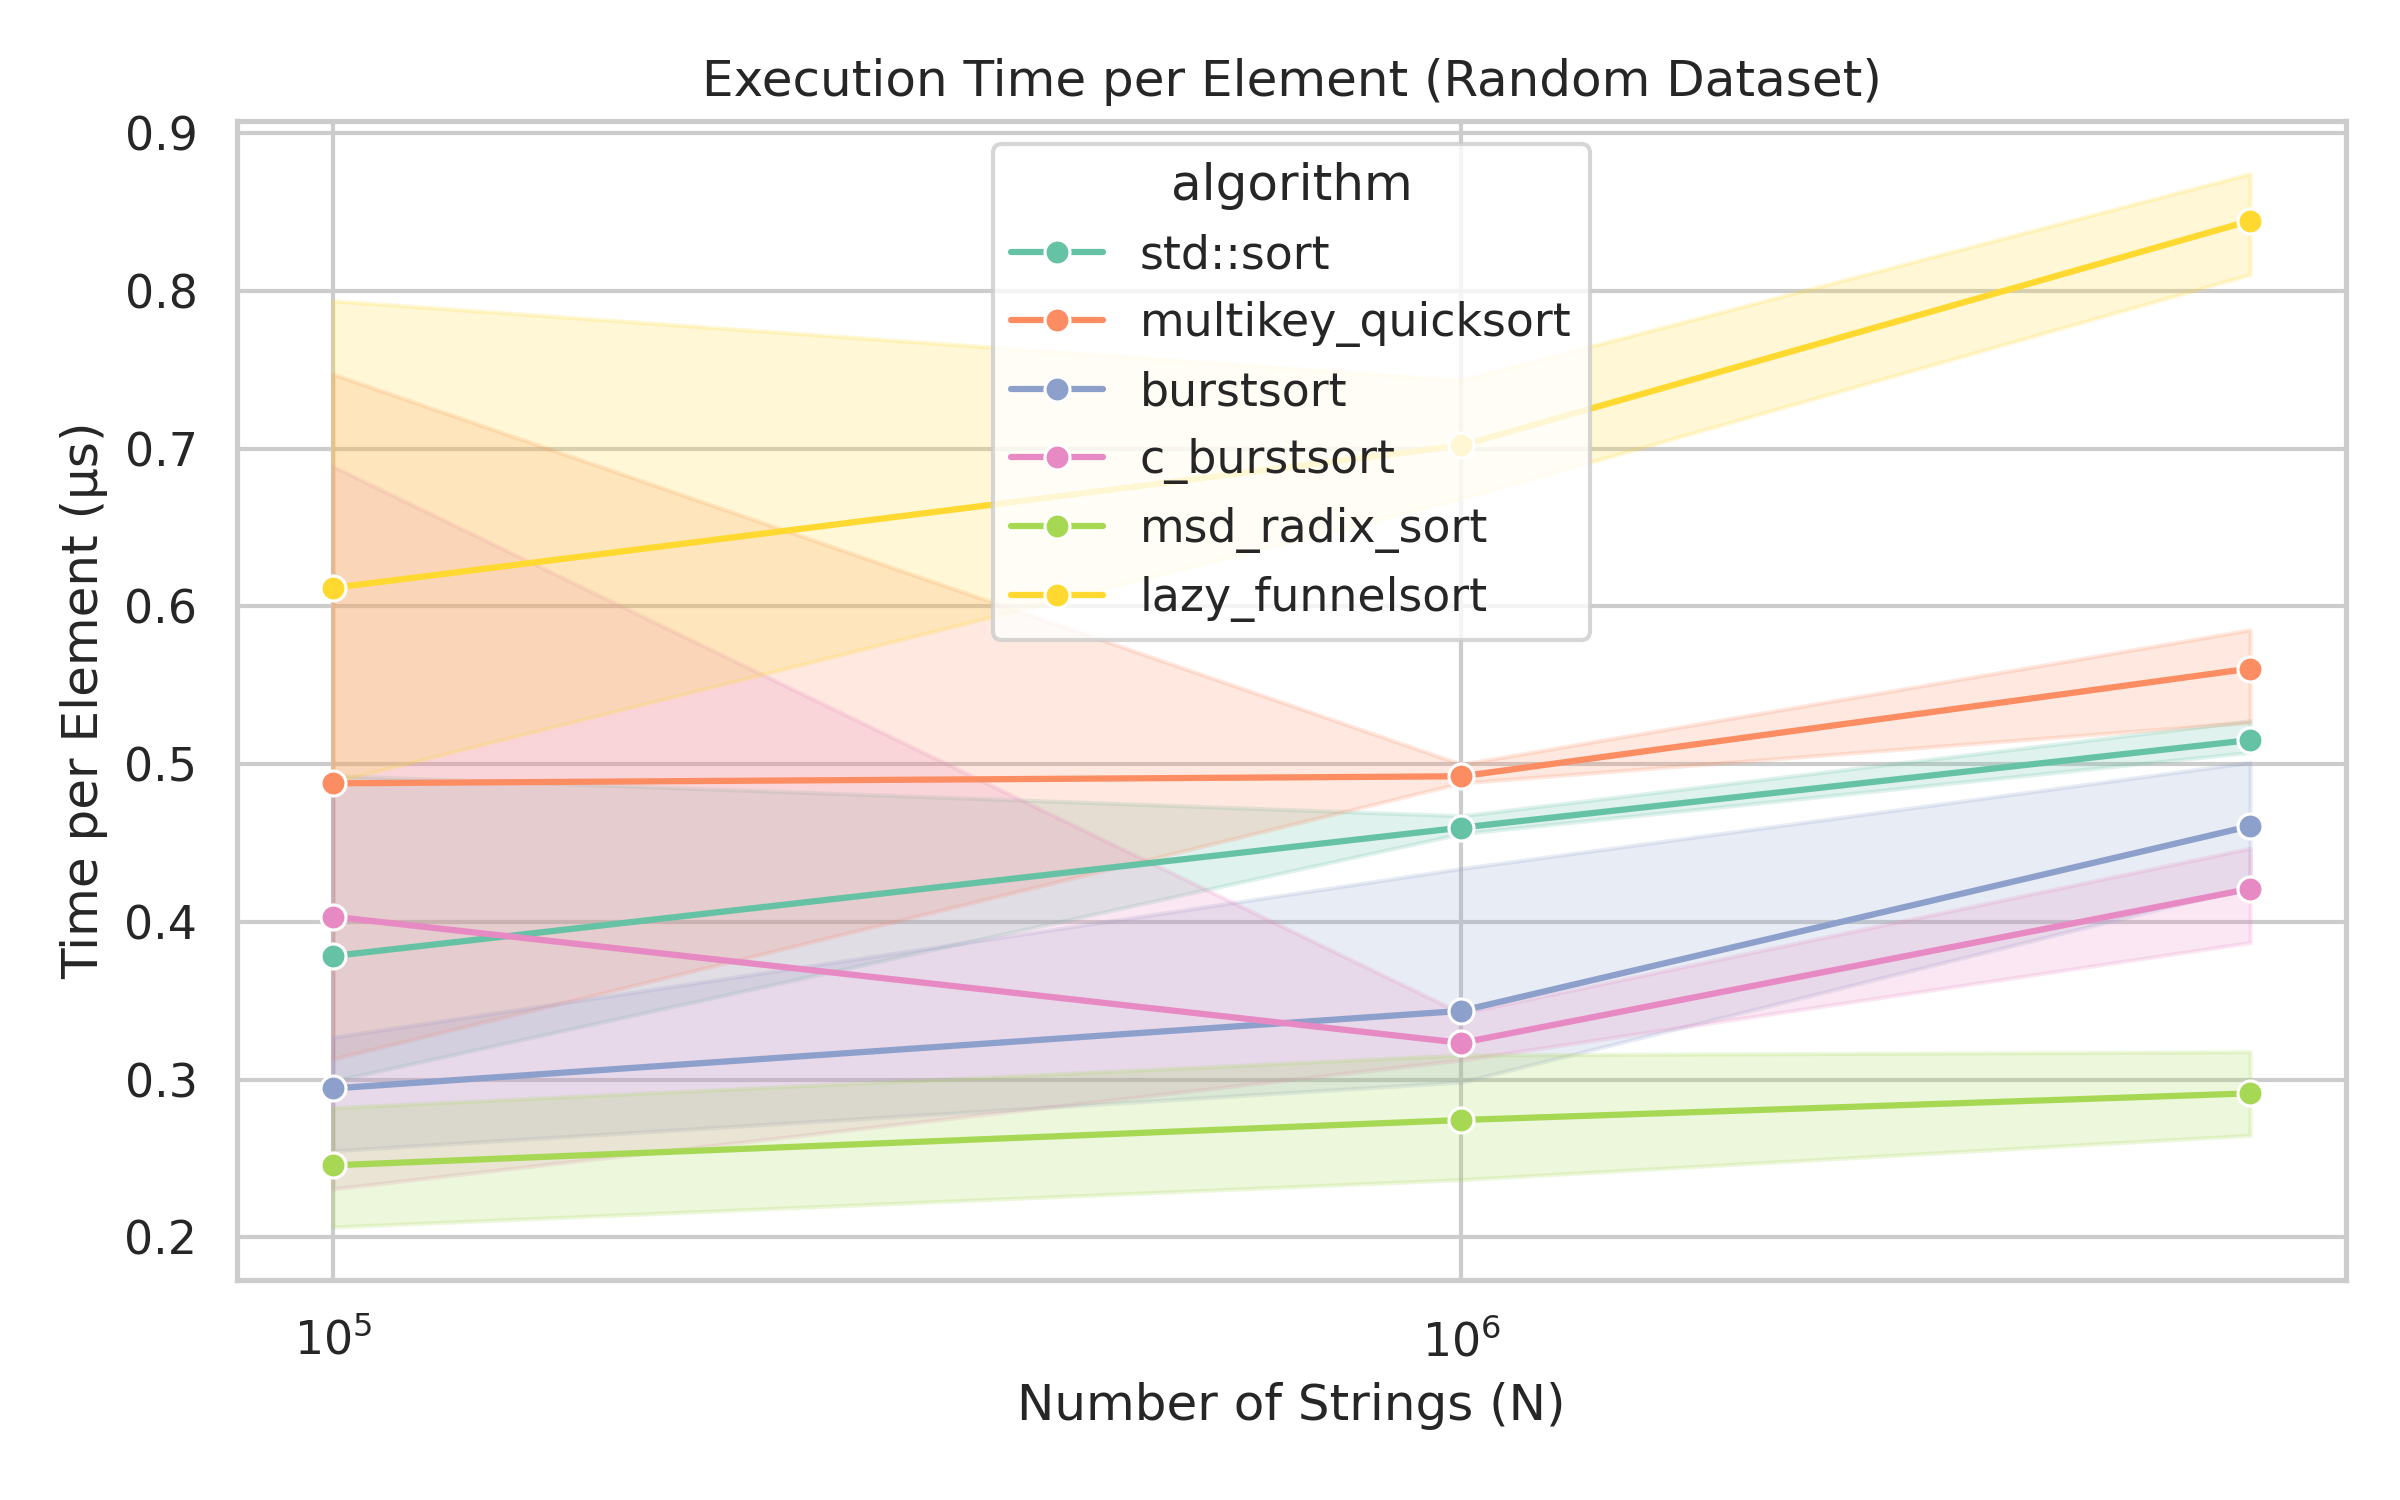
\includegraphics[width=0.8\textwidth]{Analysis/figures/time_vs_n_random.png}
    \caption{Execution Time per Element on Random Dataset.}
\end{figure}

\begin{figure}[h]
    \centering
    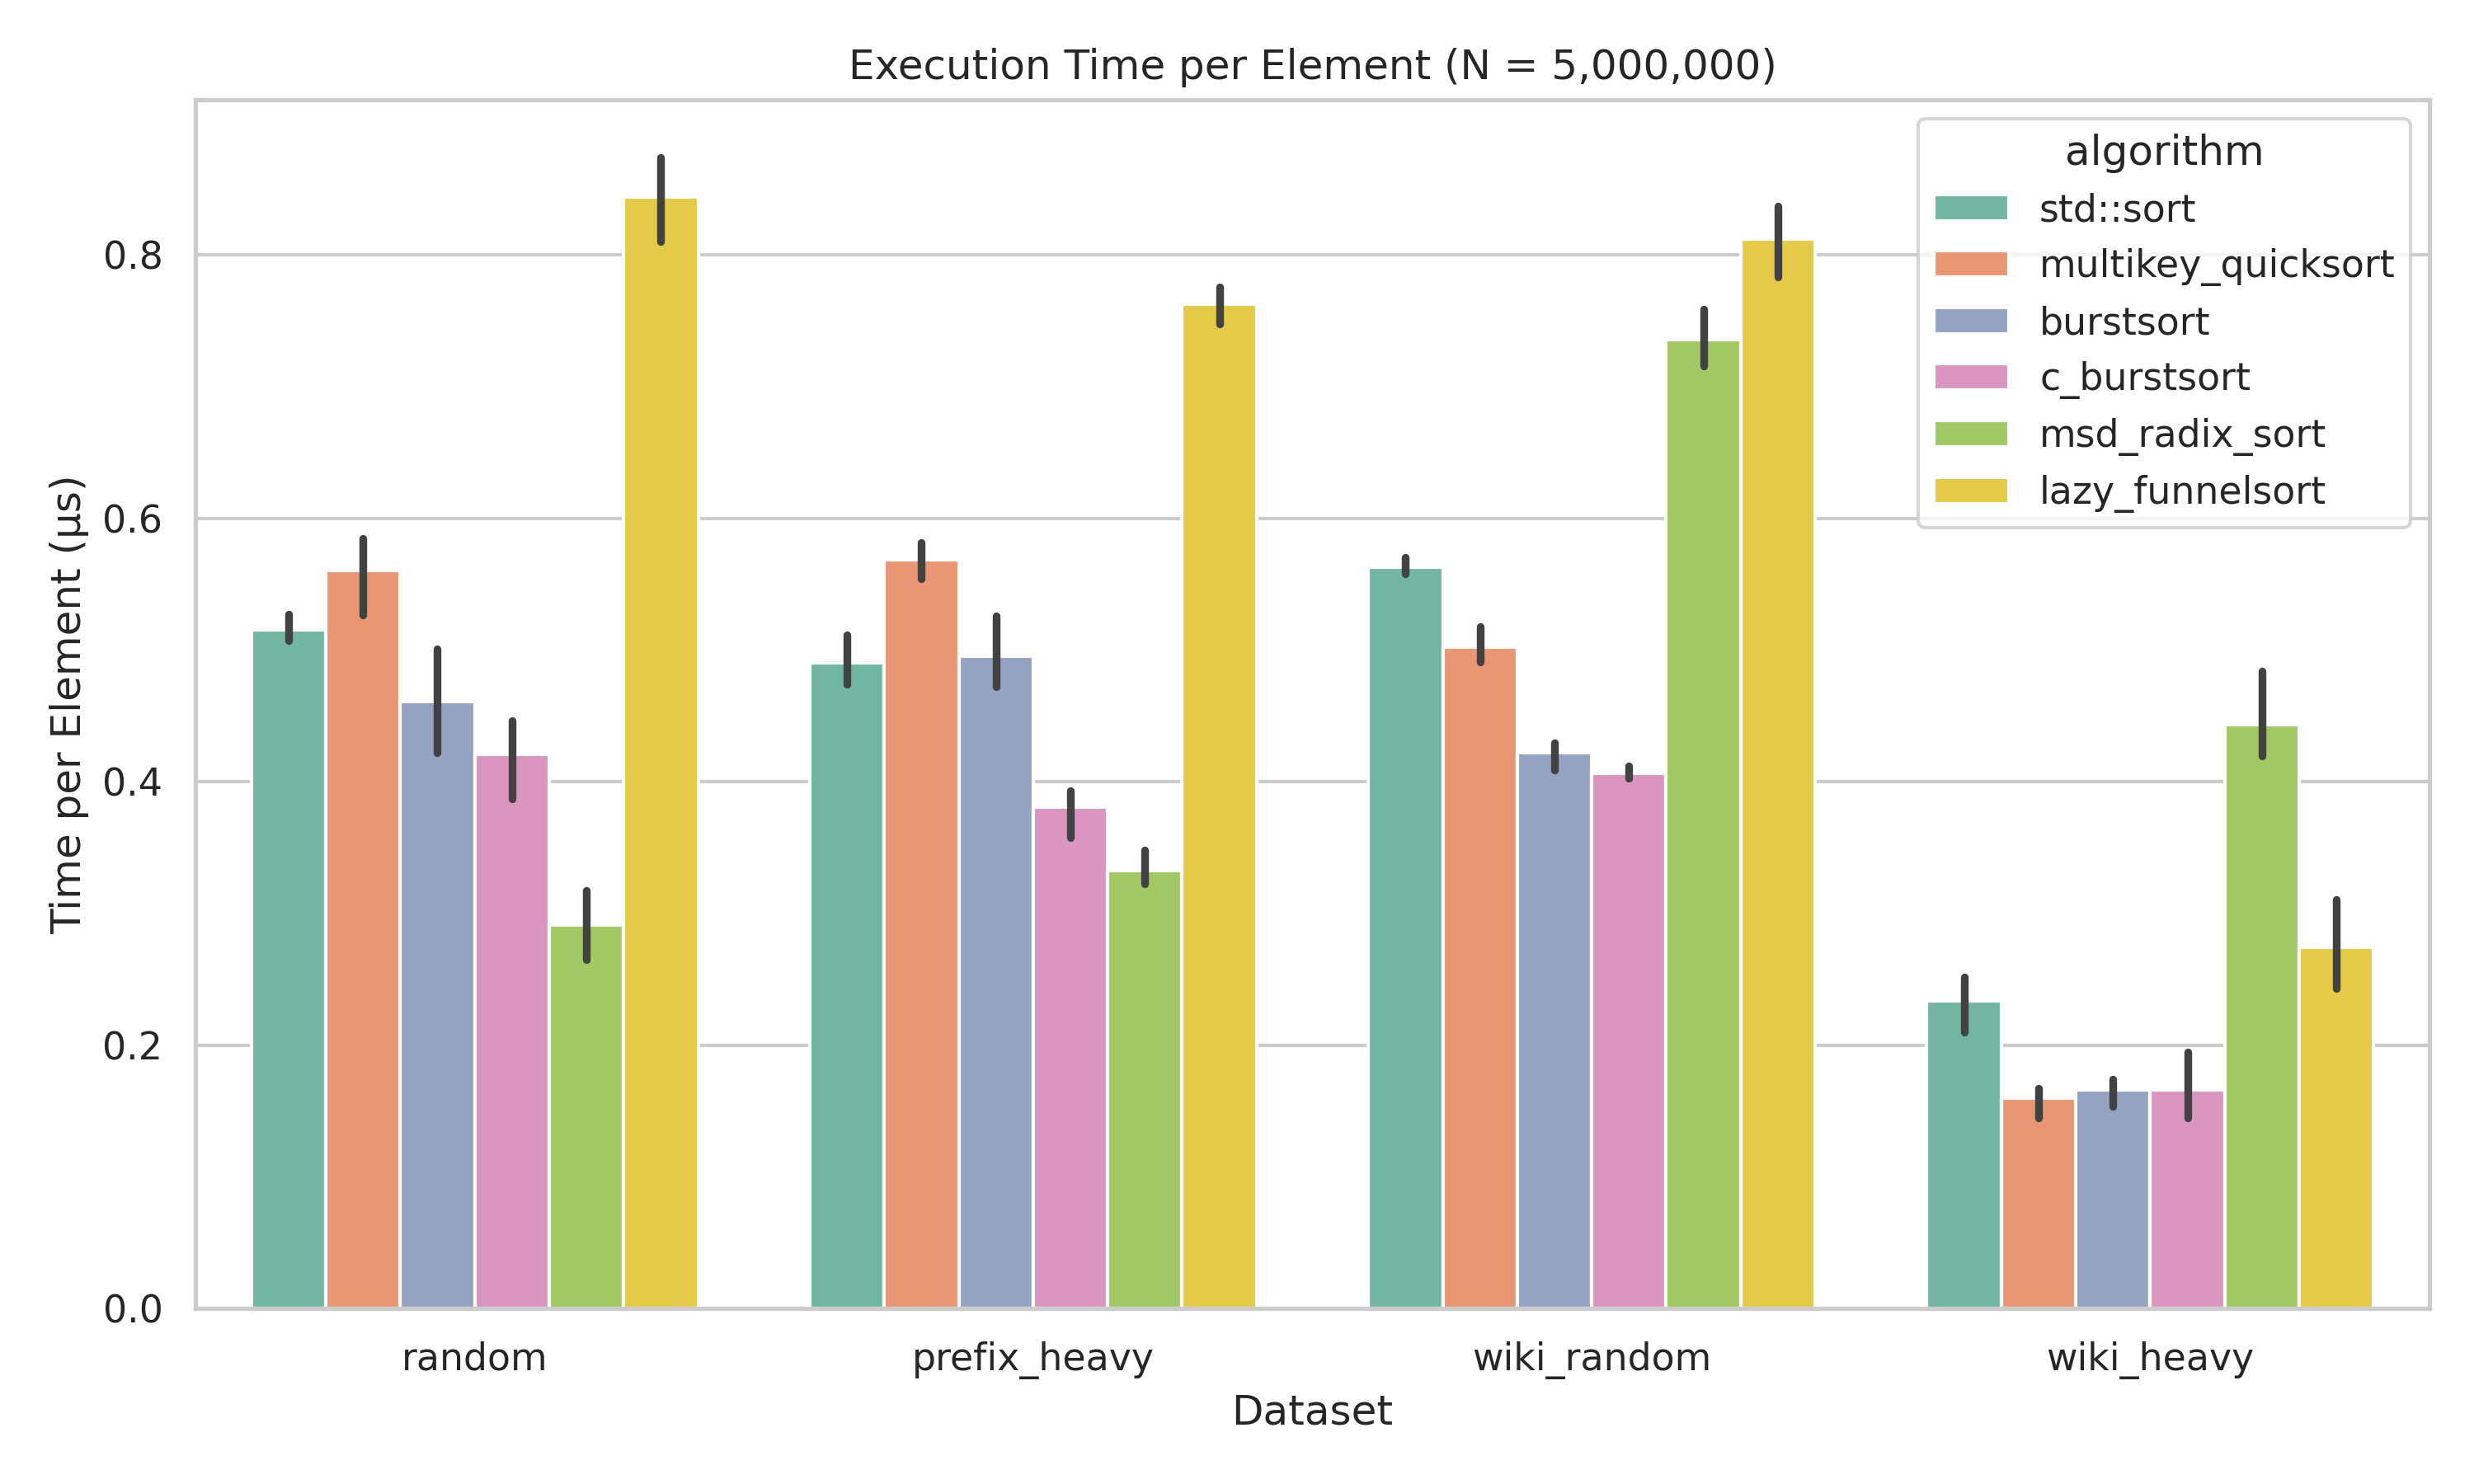
\includegraphics[width=0.8\textwidth]{Analysis/figures/bar_time_large.png}
    \caption{Execution Time per Element across all datasets for $N = 5 \times 10^6$.}
\end{figure}

\textbf{Observation:} Cache-aware algorithms like Burstsort and C-Burstsort maintain relatively flat scaling (constant time per element) for large $N$, whereas standard baseline sorts and memory-intensive approaches like MSD Radix Sort exhibit noticeable performance degradation as $N$ exceeds the LLC capacity $M$.

\subsection{Cache Profiling (L1 and LLC Misses)}
We utilized hardware performance counters to measure L1 Data Misses and LLC (Last Level Cache) Data Misses per element.

\begin{figure}[h]
    \centering
    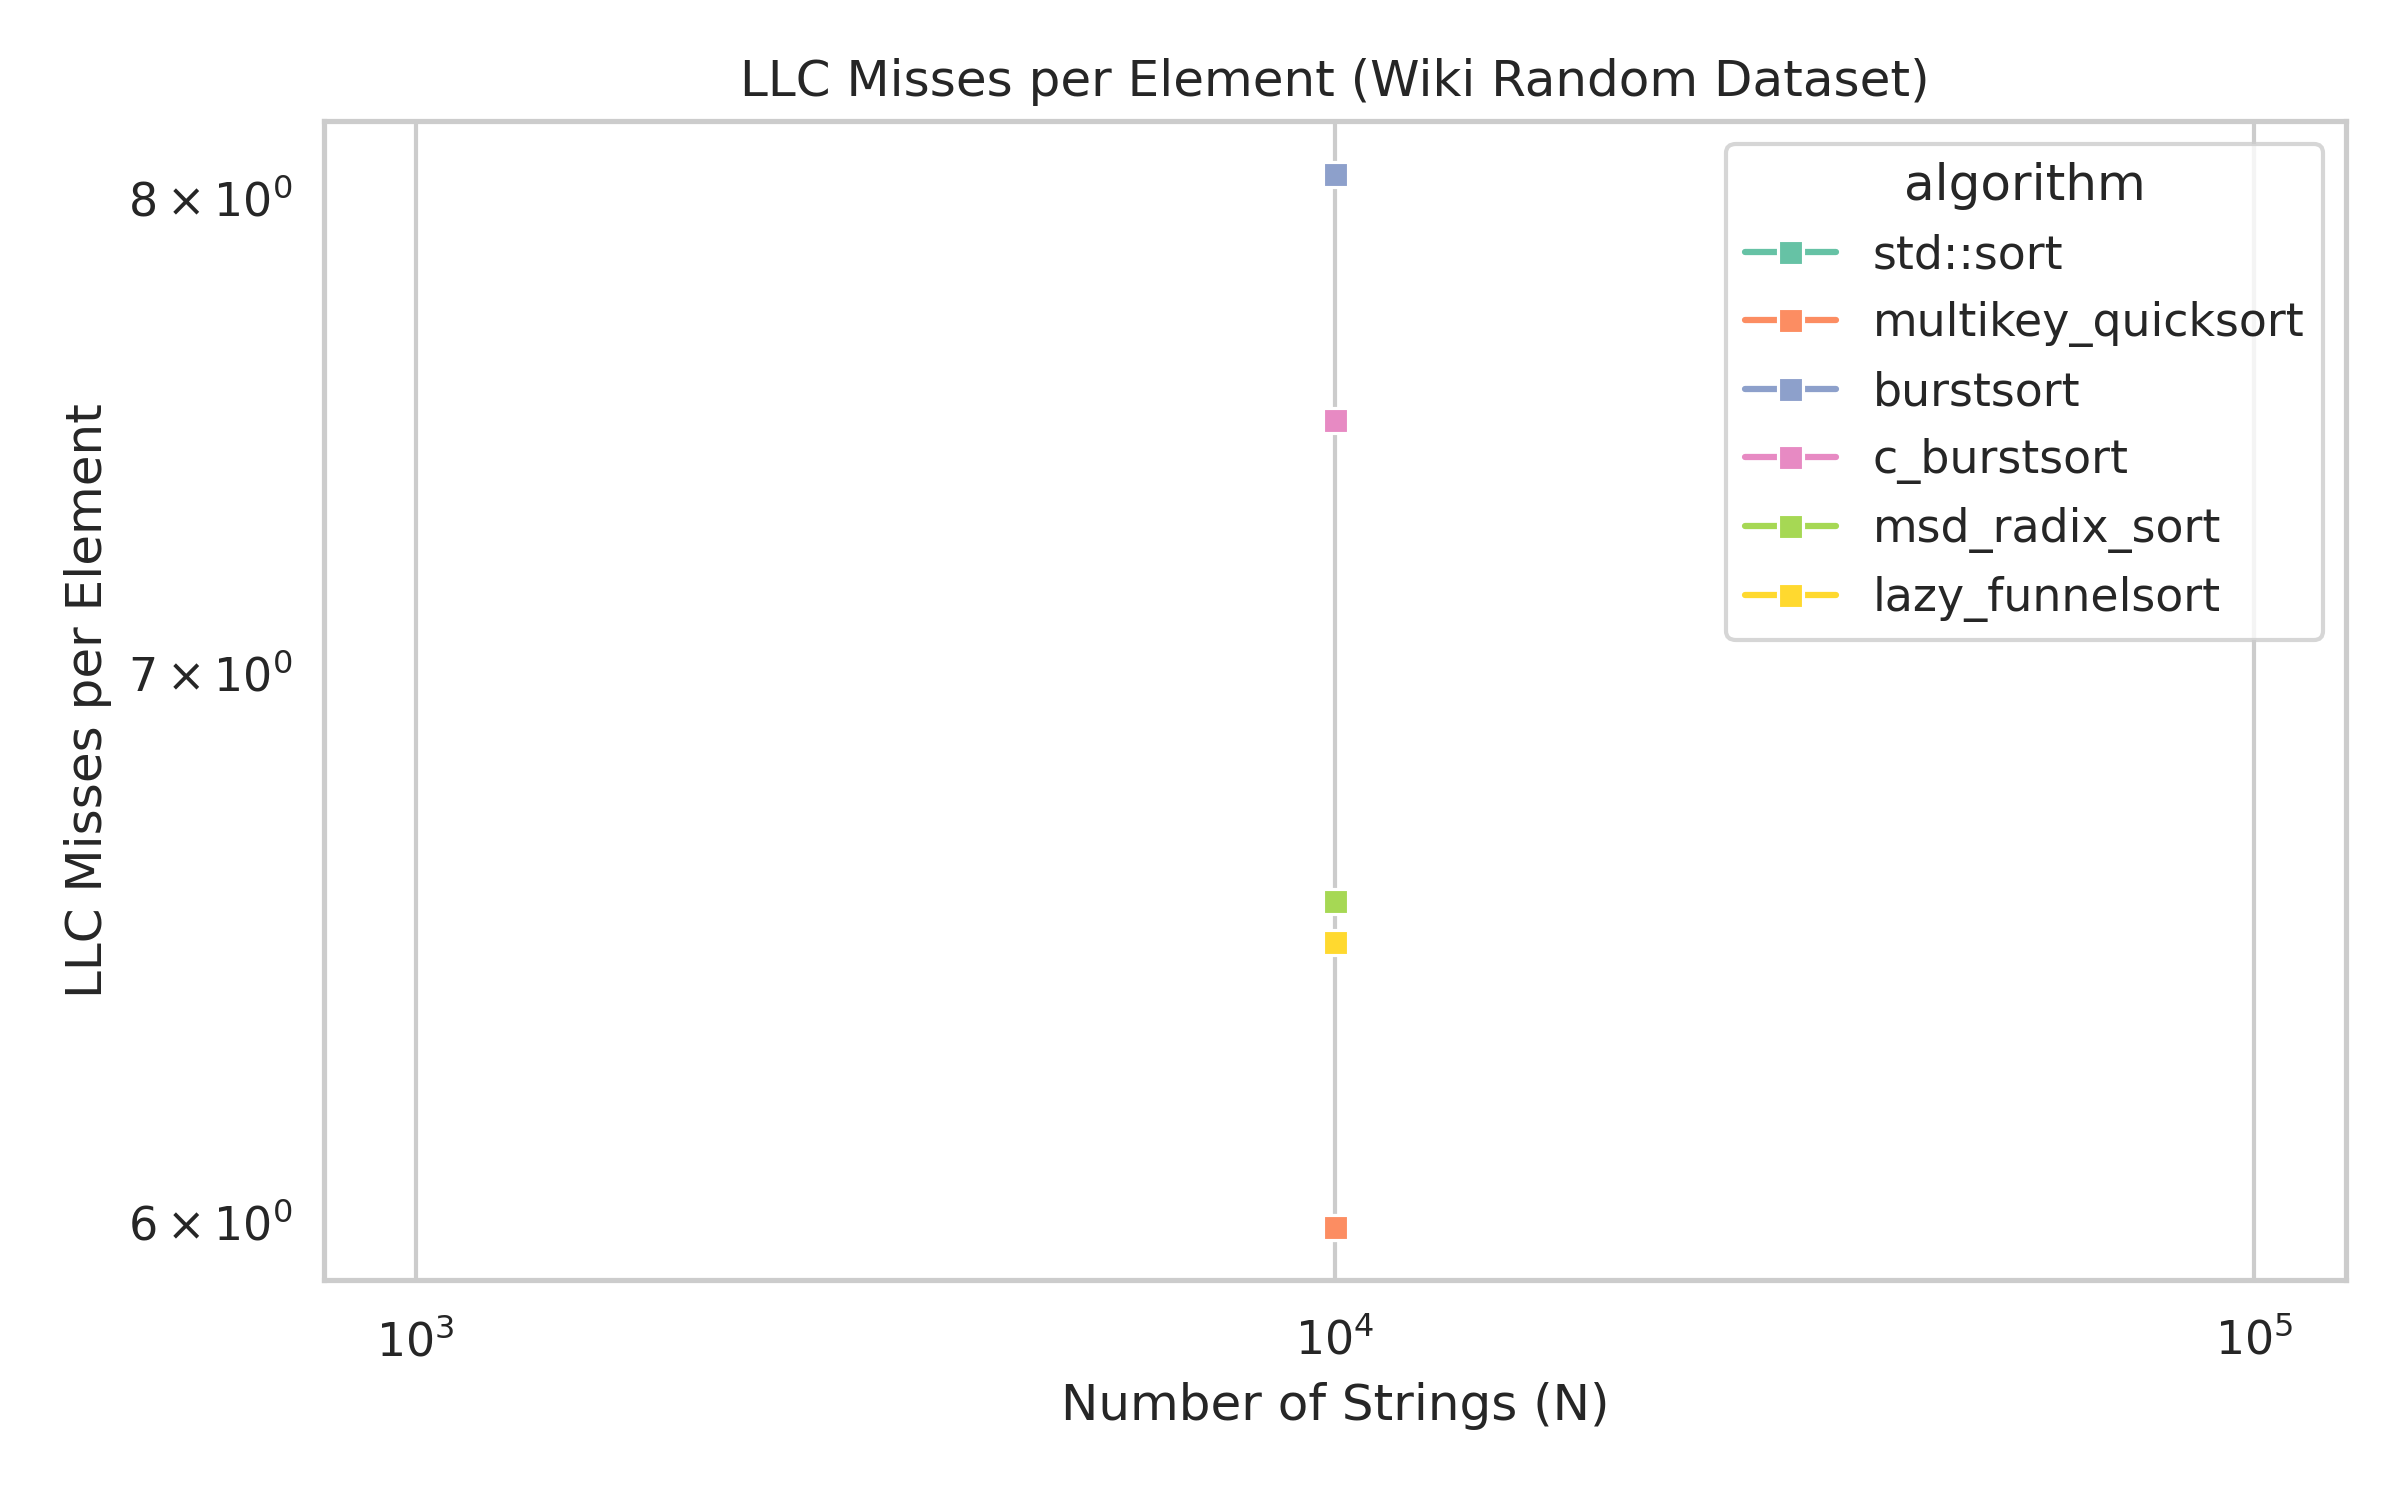
\includegraphics[width=0.8\textwidth]{Analysis/figures/llc_vs_n_wiki.png}
    \caption{LLC Misses per Element on Wiki Random Dataset.}
\end{figure}

\textbf{Observation:} MSD Radix Sort shows significantly higher miss rates due to bucket thrashing, while Burstsort remains near the theoretical scanning limit, demonstrating its superior cache utilization.

\section{Codebase Architecture}
The project is implemented in \textbf{C++20} for high-performance memory management and deterministic cache control.

\subsection{File Structure}
\begin{itemize}
    \item \texttt{main.cpp}: Entry point; manages dataset generation, loading, and the benchmarking loop.
    \item \texttt{algorithms/}: Contains implementation headers and source files.
    \begin{itemize}
        \item \texttt{radix.cpp}: MSD Radix Sort implementation.
        \item \texttt{burstsort.cpp}: Optimized C-Burstsort using an arena-based memory model.
        \item \texttt{baselines.cpp}: implementations of MKQS and \texttt{std::sort} wrappers.
    \end{itemize}
    \item \texttt{Analysis/}: Python scripts (\texttt{update\_nbs.py}) and Jupyter notebooks for data visualization using Seaborn and Matplotlib.
\end{itemize}

\end{document}